\documentclass[letterpaper,12pt]{article}
\usepackage[utf8]{inputenc}
\usepackage[top=1.25in, bottom=1.25in, left=1in, right=1in]{geometry}
\usepackage{amsmath}
\usepackage{amsfonts}
\usepackage{enumitem}
\usepackage{graphicx}

\setenumerate{parsep=0em, listparindent=\parindent}

\DeclareMathOperator{\Tr}{Tr}
\DeclareMathOperator{\dom}{dom}
\DeclareMathOperator{\diag}{diag}
\DeclareMathOperator{\dist}{dist}

\title{Homework 3}
\author{Benjamin Noland}
\date{}

\begin{document}

\maketitle

\begin{enumerate}
\item Below is the uncorrected (i.e., corrupted) image:
  \begin{center}
    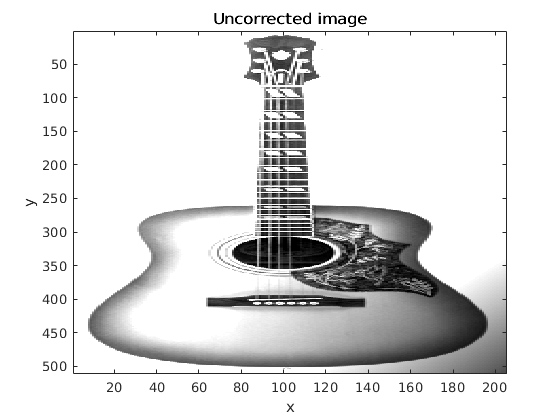
\includegraphics[width=10cm]{uncorrected_image.png}
  \end{center}
  In order to remove the corruption from this image, we want to fit a
  model of the form
  \begin{equation*}
    e_c(i, j) = r(i, j) e(i, j),
  \end{equation*}
  where $e_c(i, j)$ is the corrupted image, $e(i, j)$ is the true
  (uncorrupted) image, and $r(i, j) = ai + bj + c$ is an affine
  function of the pixel coordinates $(i, j)$, satisfying
  $|r(i, j)| \leq 1$. The goal is to estimate the parameters $a, b$,
  and $c$. In addition, we know that the true (uncorrupted) image
  $e(i, j)$ satisfies
  \begin{equation*}
    e(i, j) = 255 \quad \text{for every $1 \leq i < 50$ and $1 \leq j < 250$}.
  \end{equation*}
  We can use this information to find suitable values for $a, b$, and
  $c$. Specifically, we solve the (convex) optimization problem
  \begin{align*}
    &\text{minimize} \
      \sum_{i=1}^{49} \sum_{j=1}^{249} (e_c(i, j) - 255 r(i, j))^2 \\
    &\text{subject to} \ |r(i, j)| \leq 1.
  \end{align*}
  Finally, we compute an estimate $\hat{e}(i, j)$ of the true
  (uncorrupted) image by computing
  $\hat{e}(i, j) = e_c(i, j) / r(i, j)$ for all pixel coordinates
  $(i, j)$.

  Running the code, we get the following output from the convex
  optimization procedure:
  \begin{verbatim}
Status: Solved
Optimal value (cvx_optval): +32.0336
  \end{verbatim}
  and the following coefficient estimates:
  \begin{verbatim}
Optimal values:
a = -0.00099997
b = -0.0020002
c = 0.99824
  \end{verbatim}
  Below is the resulting corrected image:
  \begin{center}
    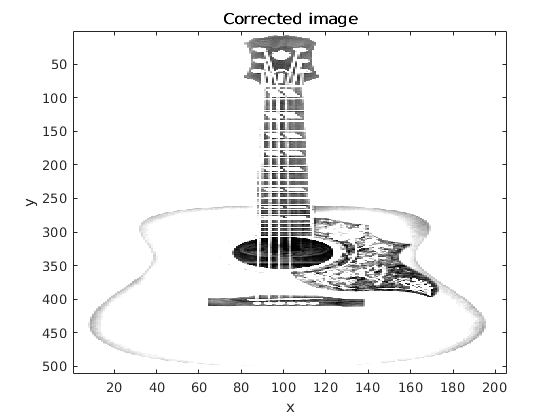
\includegraphics[width=10cm]{corrected_image.png}
  \end{center}

\item We have raw data points $X$ and $Y$, which consist of ordered
  collections $X = (x_1, \ldots, x_N)$ and $Y = (y_1, \ldots, y_N)$ of
  corresponding $x$- and $y$-coordinates, respectively.

  First, we divide these collections into $M$ disjoint segments of $K$
  coordinates each: $X_1, \ldots, X_M$ of $x$-coordinates and
  $Y_1, \ldots, Y_M$ of $y$-coordinates, where
  $Y_i = (y_{i1}, \ldots, y_{iK})$ is the collection of
  $y$-coordinates associated with the $x$-coordinates
  $X_i = (x_{i1}, \ldots, x_{iK})$. The reason for segments of equal
  length $K$ is to simplify the implementation.

  For each of the segments $X_i$ and $Y_i$ we want to fit cubic polynomials
  \begin{align*}
    x_i(t) &= a_{i3}t^3 + a_{i2}t^2 + a_{i1}t + a_{i0} \\
    y_i(t) &= b_{i3}t^3 + b_{i2}t^2 + b_{i1}t + b_{i0},
  \end{align*}
  respectively, each of which is parameterized by a variable
  $t \in [0, 1]$. For each segment we fit the polynomial via least
  squares, subject to second-order smoothness
  constraints. Specifically, we require that, for every $1 \leq i < M$,
  \begin{equation*}
    \begin{aligned}
      x_i(1) &= x_{i+1}(0) \\
      x_i'(1) &= x_{i+1}'(0) \\
      x_i''(1) &= x_{i+1}''(0)
    \end{aligned}
    \quad \text{and} \quad
    \begin{aligned}
      y_i(1) &= y_{i+1}(0) \\
      y_i'(1) &= y_{i+1}'(0) \\
      y_i''(1) &= y_{i+1}''(0).
    \end{aligned}
  \end{equation*}
  Written in terms of the polynomial coefficients $a_{ij}$ and
  $b_{ij}$, these constraints become
  \begin{align} \label{eq:a_constraints}
    \begin{split}
      a_{i3} + a_{i2} + a_{i1} + a_{i0} &= a_{i+1,0} \\
      3a_{i3} + 2a_{i2} + a_{i1} &= a_{i+1,1} \\
      6a_{i3} + 2a_{i2} &= 2a_{i+1,2}
    \end{split}
  \end{align}
  \begin{align} \label{eq:b_constraints}
    \begin{split}
      b_{i3} + b_{i2} + b_{i1} + b_{i0} &= b_{i+1,0} \\
      3b_{i3} + 2b_{i2} + b_{i1} &= b_{i+1,1} \\
      6b_{i3} + 2b_{i2} &= 2b_{i+1,2}
    \end{split}
  \end{align}
  for every $1 \leq i < M$.

  We therefore want to solve two (convex) optimization problems: one
  to compute the coefficients $a_{ij}$ and one to compute the
  coefficients $b_{ij}$, subject to the constraints
  (\ref{eq:a_constraints}) and (\ref{eq:b_constraints}),
  respectively. Let $0 = t_1 < t_2 < \cdots < t_K = 1$ be equally
  spaced elements of $[0, 1]$. To compute the coefficients $a_{ij}$,
  we solve the problem
  \begin{align*}
    &\text{minimize} \ \sum_{i=1}^M \sum_{j=1}^K (x_{ij} - x_i(t_j))^2 \\
    &\text{subject to} \ (\ref{eq:a_constraints}).
  \end{align*}
  To compute the coefficients $b_{ij}$, we solve the problem
  \begin{align*}
    &\text{minimize} \ \sum_{i=1}^M \sum_{j=1}^K (y_{ij} - y_i(t_j))^2 \\
    &\text{subject to} \ (\ref{eq:b_constraints}).
  \end{align*}
  Thus we obtain a collection of curves $(x_i(t), y_i(t))$,
  $1 \leq i \leq M$, in the plane that together form a cubic spline
  approximating the raw data points $X$ and $Y$.

  Running the code, we get the following output from the convex
  optimization procedure for fitting the $a_{ij}$ values:
  \begin{verbatim}
Status: Solved
Optimal value (cvx_optval): +220.954
  \end{verbatim}
  The following is the output from fitting the $b_{ij}$ values:
  \begin{verbatim}
Status: Solved
Optimal value (cvx_optval): +178.677
  \end{verbatim}
  Below is a plot of the $X$ and $Y$ data points (displayed in white),
  along with the fitted spline (with different segments having
  different colors):
  \begin{center}
    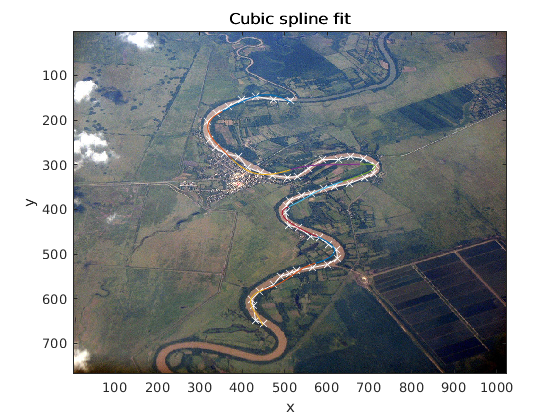
\includegraphics[width=15cm]{spline.png}
  \end{center}

\end{enumerate}

\end{document}
